\begin{frame}{Algoritmo Prism
\begin{itemize}
	\item Para cada classe \textit{c} de 1 a \textit{n}:
	\begin{itemize}
		\item \textbf{Passo 1} - Calcular a probabilidade de ocorr�ncia da classe c para cada par-atributo-valor
		\item \textbf{Passo 2} - Selecionar o pa-atributo com a probabilidade m�xima de ocorr�ncia e crie um subconjunto de treinamento tomado como entrada compreendendo todas as inst�ncias que o par selecionado (para todas as classes)
		\item \textbf{Passo 3} - Repetir os passos 1 e 2 para este subconjunto at� o momento em que ele apresente apenas inst�ncias da classe c. A regra induzida � ent�o a conjun�ao de todos os pares atributo-valor selecionados na cria�ao deste subconjunto homog�neo.
		\item \textbf{Passo 4} - Remover todas as inst�ncias, que satisfa�am a regra formada, do conjunto de treinamento.
		\item Repetir a sequ�ncia de 1 a  at� que todas as inst�ncias da classe \textit{c} tenham sido removidas.
	\end{itemize}
\end{itemize}
\end{frame}

\begin{frame}{Exemplo - parte I}
\begin{figure}
	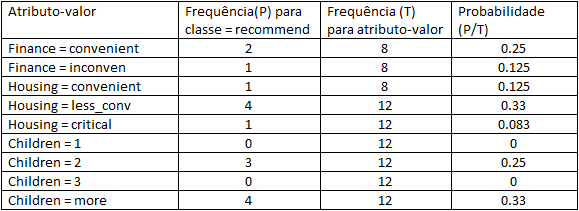
\includegraphics[scale=1]{prismaTabela1.png}
\end{figure}
\end{frame}

\begin{frame}{Exemplo - parte II}
\begin{figure}
	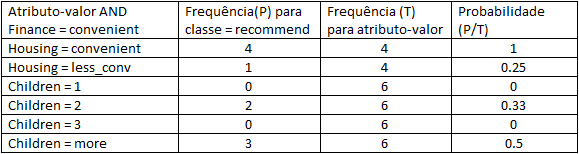
\includegraphics[scale=1]{prismaTabela2.png}
\end{figure}
\end{frame}